\chapter{B2}

{\LARGE Consider the two files and represent in a 2D chart the geographic position of the IP addresses outside the domain computed in a.3.}

\section{Explicação do código desenvolvido}

Para o desenvolvimento deste tópico decidimos utilizar a API de Geolocalização \cite{API} que nos forneceu algum código (IPGeolocation.py) de modo a facilitar a sua utilização. Na figura 8.1 pode-se ver o código criado por nós para a conversão dos IP's por localização geográfica. 

Dado que a API só nos deixava utilizar alguns recursos por dia, fomos obrigados a utilizar duas contas para gerar duas chaves de modo a cobrir o nosso código com o maior número de testes possível. Esta função \textit{getGeoLocation(ips\_addrs)} recebe um conjunto de IP's (já computados previamente) e converte-os para uma localização geográfica. Utilizamos mais uma vez um mapa para sabermos quantas vezes aparecem IP's de uma dada localização, sendo este mapa no fim ordenado da localidade mais utilizada, para a menos utilizada.


\begin{figure}[h!]
    \label{high}
    \centering
    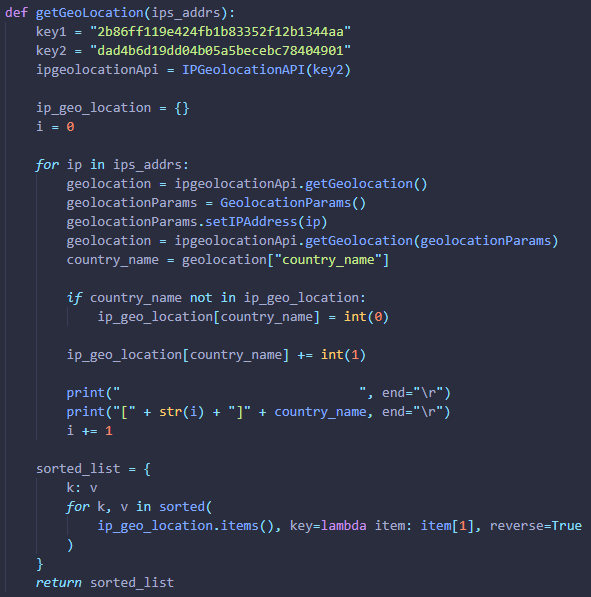
\includegraphics[width=0.7\textwidth]{Images/b2/getGeoLocation.png}
    \caption{\textit{Código do tópico b2}}
\end{figure}

Na figura 8.2 podemos verificar como esta função é utilizada depois da computação dos IP's e a forma como essa informação é ordenada.

\begin{figure}[h!]
    \label{high}
    \centering
    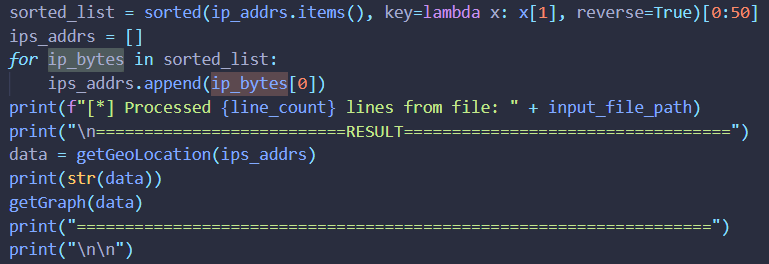
\includegraphics[width=0.7\textwidth]{Images/b2/result.png}
    \caption{\textit{\textit{Print} e gráfico do resultado b2}}
\end{figure}

Passando agora à analise do código que itera todas as linhas do ficheiro, podemos verificar que o código é muito simples de se entender. Inicialmente inicializamos as variáveis úteis, e caso se trate de um fluxo exterior (de origem ou destino) inicializamos a nossa estrutura de dados (mapa) e adicionamos o IP's associado. 

\begin{figure}[h!]
    \label{high}
    \centering
    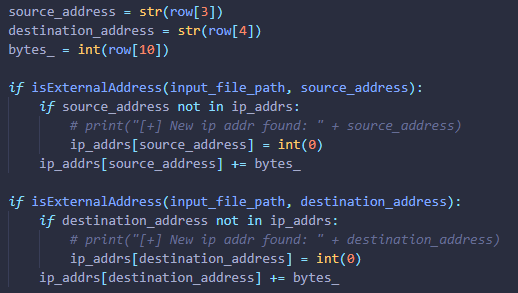
\includegraphics[width=0.9\textwidth]{Images/b2/b2.png}
    \caption{\textit{Código do tópico b2}}
\end{figure}

%----------------------------------------------------------------------------
%----------------------------------------------------------------------------
\newpage

\section{Resultados obtidos pelo ficheiro www.fct.unl.pt.csv}

Para os resultados do ficheiro www.fct.unl.pt.csv era de esperar que Portugal dominasse como localização mais comum entre os IP's. Nas figuras 8.4 e 8.5 podemos ver os resultados em forma de gráfico e em forma de mapa. 

\begin{figure}[h!]
    \label{high}
    \centering
    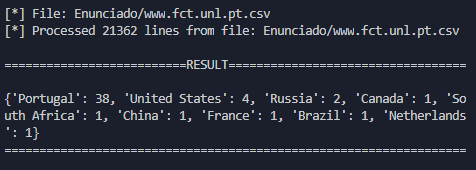
\includegraphics[width=1\textwidth]{Images/b2/b2_a.png}
    \caption{\textit{Output do script b2.py}}
\end{figure}

\begin{figure}[h!]
    \label{high}
    \centering
    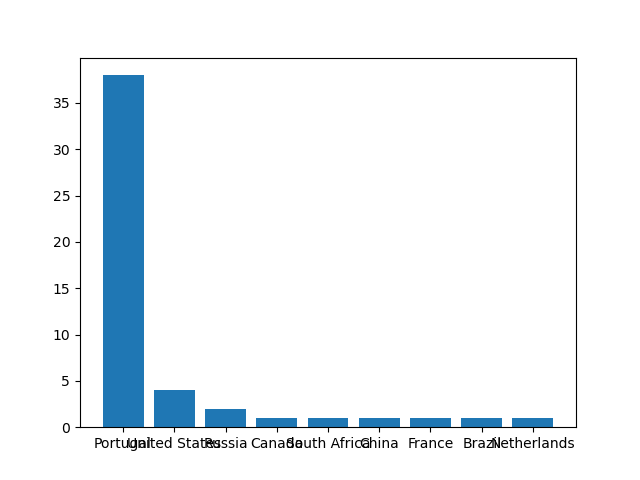
\includegraphics[width=1\textwidth]{Images/b2/b2_1.png}
    \caption{\textit{Gráfico das posições geográficas do endereços IP}}
\end{figure}

\clearpage

\section{Resultados obtidos pelo ficheiro bigFlows.csv}

Para os resultados do ficheiro bigFlows.csv os Estados Unidos dominam consideravelmente, estando os resultados apresentados nas figuras 8.6 e 8.7 seguintes.

\begin{figure}[h!]
    \label{high}
    \centering
    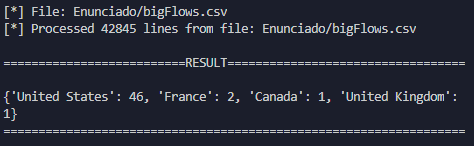
\includegraphics[width=1\textwidth]{Images/b2/b2_b.png}
    \caption{\textit{Output do script b2.py}}
\end{figure}

\begin{figure}[h!]
    \label{high}
    \centering
    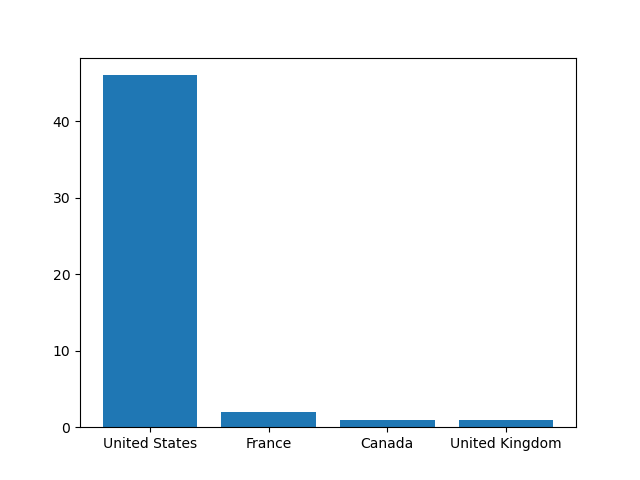
\includegraphics[width=1\textwidth]{Images/b2/b2_2.png}
    \caption{\textit{Gráfico das posições geográficas do endereços IP}}
\end{figure}